\documentclass{uofa-eng-assignment}

\usepackage{lipsum}

\newcommand*{\name}{Tachibana Kanade}
\newcommand*{\id}{1234567890}
\newcommand*{\course}{Dating 101}
\newcommand*{\assignment}{Assignment 1}
\usepackage{listings}

\begin{document}



\maketitle

\begin{enumerate}

%%%%%%%%%%%%%%%%%%%%
\item Question Number 1
%%%%%%%%%%%%%%%%%%%%

\textbf{Solution.}

Let $f(x) = z^3 - z^2 + z - 1, z\in \mathbb{C}$. 
The derivative of $f$ is $f'(z) = 3z^2 - 2z + 1$

By Newton's method, 
\[z_{n + 1} = z_{n} - \frac{f(z_{n})}{f'(z_{n})} = z_{n} - \frac{z_n^3-z_n^2+z_n-1}{3z_n^2-2z_n + 1}\]

where $z_0 \in R:= [-2, 2] \times [-2, 2]$

The following python code solves this one.

\begin{lstlisting}[language=python]
def newton_iteration(z0):
		zn = z0 # z_{n}
		zn_1 = z0 + 1 # z_{n-1}
		tolerance = 10 ** -6
		max_iteration = 20
		while abs(zn_1 - zn) > tolerance and max_iteration > 0:
			numerator = (zn ** 3) - (zn ** 2) + zn - 1
			denominator = 3 * (zn ** 2) - 2 * zn + 1
			zn_1 = zn
			zn -= numerator/denominator
			max_iteration -= 1
		return (zn, 20 - max_iteration)

def solving_equation(): # question (a)
    chunk = 4 / 401
    X = []
    Y = []
    Z = []
    color = []
    for i in range(401):
        for j in range(401):

            px = random.uniform(-2 + chunk * i, -2 + chunk * (i + 1))
            py = random.uniform(-2 + chunk * j, -2 + chunk * (j + 1))
    
            (z, N) = newton_iteration(complex(px, py))
            X.append(px)
            Y.append(py)
            color.append(N)
            Z.append(z)

    return (X, Y, color, Z)
	\end{lstlisting}

%%%%%%%%%%%%%%%%%%%%
\item Question Number 2
%%%%%%%%%%%%%%%%%%%%

Roots are $1, i, -i$.
Python code:
\begin{lstlisting}[language=python]
def plot_num_iter_converge(): # question (b)
    plt.subplot()
    plt.ylabel("Im(z)")
    plt.xlabel("Re(z)")
    plt.xlim((-2, 2))
    plt.ylim((-2, 2))

    (X, Y, color, Z) = solving_equation()
    sc = plt.scatter(X, Y, c=color, label="# Iterations required to converge")
    plt.colorbar(sc, label="#iterations")
    plt.show()
\end{lstlisting}

Result:

\graphicspath{ {./images/} }
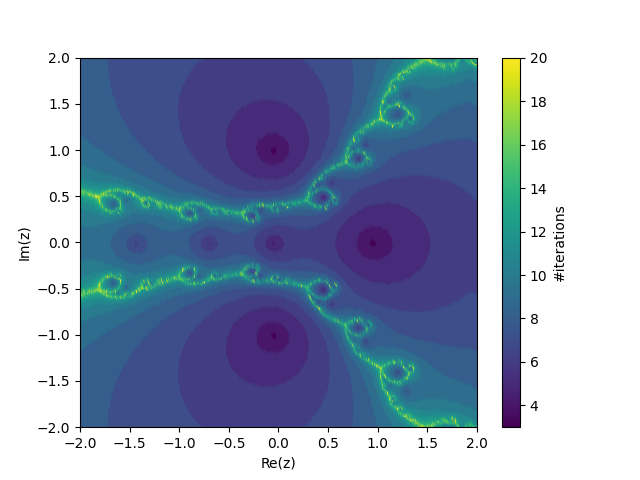
\includegraphics{./b.png}

%%%%%%%%%%%%%%%%%%%%
\item Question Number 3
%%%%%%%%%%%%%%%%%%%%

Python code:

\pagebreak
\begin{lstlisting}[language=python]
def plot_root_reach():
    plt.subplot()
    plt.ylabel("Im(z)")
    plt.xlabel("Re(z)")
    plt.xlim((-2, 2))
    plt.ylim((-2, 2))

    roots = [1, 1j, -1j]
    colors = [0,1,2]
    root_labels = ['1', 'i', '-i']

    (X, Y, color, Z) = solving_equation()

    root_color = []
    for z in Z:
        norm = [abs(z - root) for root in roots]
        index, _ = min(enumerate(norm), key=itemgetter(1))
        root_color.append(colors[index])
    
    sc = plt.scatter(X, Y, c=root_color, label="#Root converge plot")
    plt.colorbar(sc,label="#root converge", format=ticker.FuncFormatter(lambda x, y: root_labels[floor(x)]))
    plt.show()
\end{lstlisting}

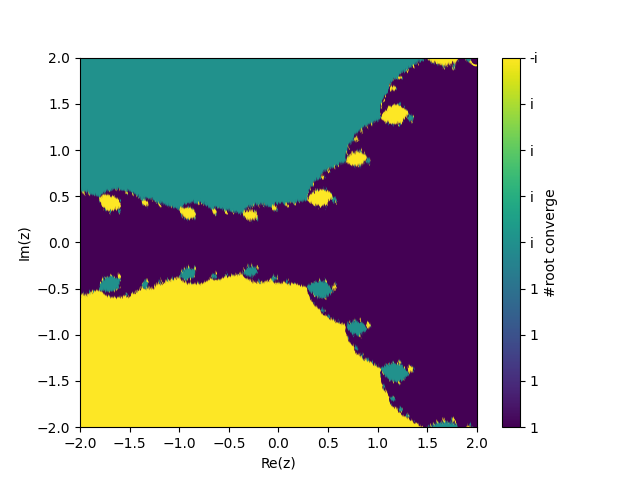
\includegraphics{./c.png}



\end{document}
